\input{mmd-beamer-header-11pt}
\def\mytitle{Part 4: Practical Bayesian methods}
\def\mydate{25 March 2015}
\def\myauthor{Matthew Pitkin}
\def\affiliation{University of Glasgow}
\def\latexxslt{beamer}
\def\latexmode{beamer}
\def\theme{m}
\def\event{GraWIToN School}
\input{mmd-beamer-begin-doc}


% Part 4 of my lecture course on statistics for the GraWIToN school
%
% Practical Bayesian methods


\begin{frame}

\frametitle{Overview}
\label{overview}

In this part of the course we will discuss a practical method for Bayesian parameter estimation:

\begin{itemize}
\item Markov chain Monte Carlo (MCMC)

\end{itemize}

This method is now very commonly used to perform parameter estimation for multi-dimensional
posterior parameter spaces.

\end{frame}

\begin{frame}

\frametitle{Markov chain Monte Carlo (MCMC)}
\label{markovchainmontecarlomcmc}

\textbf{Markov chain Monte Carlo} (MCMC)

\begin{itemize}
\item Markov chain - a sequence of random variables where the probability of a subsequent state only depends
on the current state (they are ``memoryless'')

\item Monte Carlo - an algorithm relying on repeated random sampling

\end{itemize}

So, a MCMC is a class of algorithms for drawing random samples that have a Markovian property.

We are particularly interesting in the \textbf{Metropolis-Hastings algorithm}. This can be used to efficiently
draw samples from an underlying probability distribution.

\end{frame}

\begin{frame}

\frametitle{MCMC demonstration}
\label{mcmcdemonstration}

The Metropolis-Hastings algorithm (simplified to a 1D case):

\begin{itemize}
\item choose some initial random point in the parameter space, $x_1$, and calculate posterior $p(x_1|d,I)$

\item centre a new pdf $q(x'|x_1,I)$, the \textbf{proposal distribution}, at $x_1$

\item randomly draw a point from $x_2 \sim q(x'|x_1,I)$, and calculate posterior $p(x_2|d,I)$

\end{itemize}

Now compute the ratio
\[
R = \frac{p(x_2|d,I)}{p(x_1|d,I)} \frac{q(x_2|x_1,I)}{q(x_1|x_2,I)}
\]

\end{frame}

\begin{frame}

\frametitle{MCMC demonstration}
\label{mcmcdemonstration}

The Metropolis-Hastings algorithm:

\begin{itemize}
\item accept the point $x_2$ if $R > 1$ (go uphill in posterior)

\item if $R<1$

\begin{itemize}
\item accept the point $x_2$ with a probability $R$ (go downhill in posterior)

\item otherwise reject the new point $x_2$ and set $x_2 = x_1$

\end{itemize}

\end{itemize}

This process gets repeated many times to build up a chain of samples.

Note: in general the proposal distribution will be Gaussian, so will be symmetric and
$\frac{q(x_2|x_1,I)}{q(x_1|x_2,I)} = 1$. This ratio is required to maintain \textbf{detailed balance},
i.e. there should be the same probability to go forward along the chain as to run it in reverse.

\end{frame}

\begin{frame}

\frametitle{MCMC demonstration}
\label{mcmcdemonstration}

\begin{figure}[htbp]
\centering
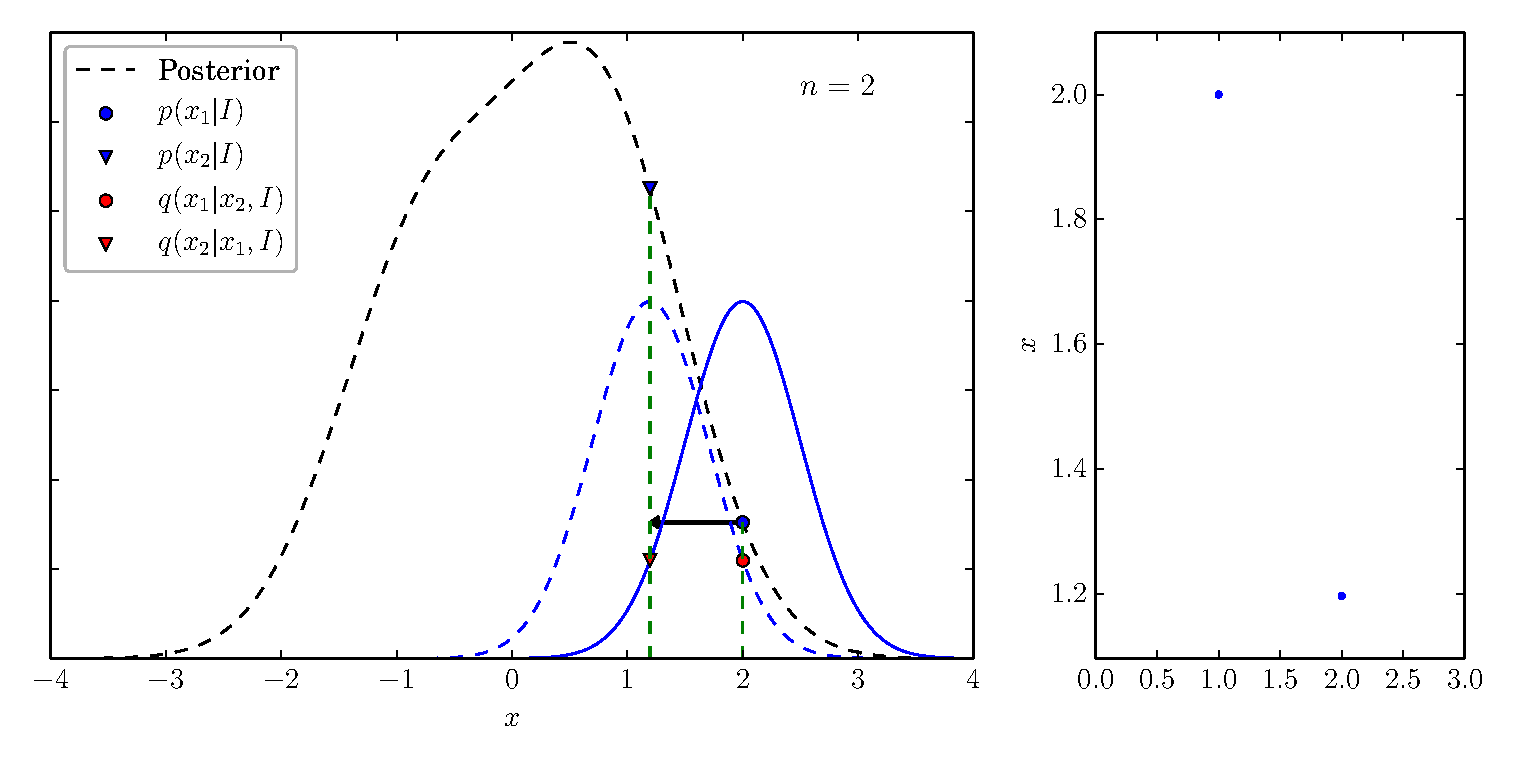
\includegraphics[keepaspectratio,width=\textwidth,height=250pt]{figures/mcmc_example_1.pdf}
\label{mcmc_example_1}
\end{figure}

\end{frame}

\begin{frame}

\frametitle{MCMC demonstration}
\label{mcmcdemonstration}

So the Metropolis Algorithm generally (but not always) moves uphill, towards the peak
of the posterior pdf.

\emph{Remarkable facts}:

\begin{itemize}
\item The sequence of points $\{x_1, x_2, \ldots, x_n\}$ represent samples from the marginalised
posterior $p(x|d,I)$

\item We can make a histogram of $\{x_1, x_2, \ldots, x_n\}$ and use it to compute the mean and variance
of $x$

\end{itemize}

\end{frame}

\begin{frame}

\frametitle{MCMC demonstration}
\label{mcmcdemonstration}

\begin{figure}[htbp]
\centering
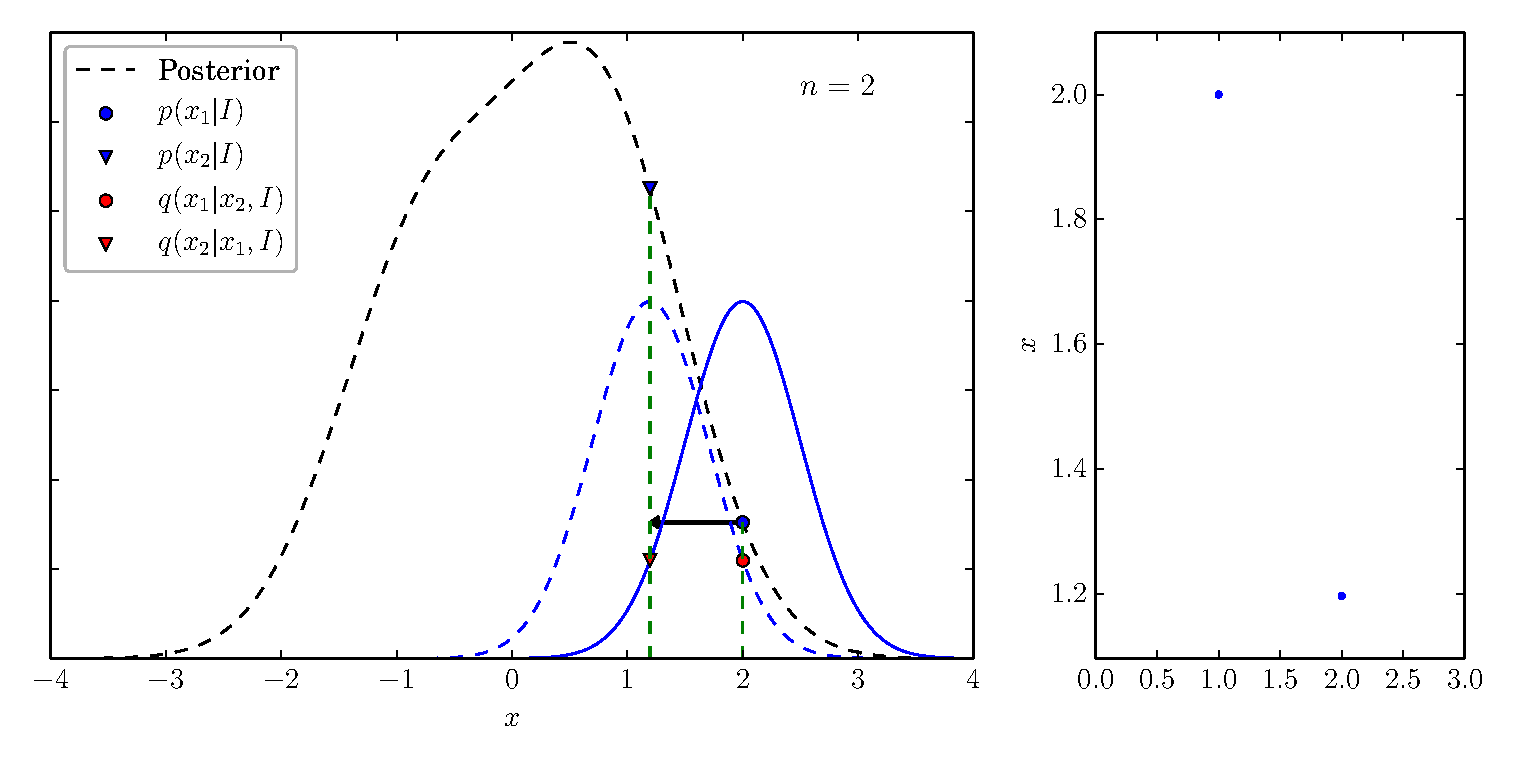
\includegraphics[keepaspectratio,width=\textwidth,height=250pt]{figures/mcmc_example_1.pdf}
\label{mcmc_example_1}
\end{figure}

\end{frame}

\begin{frame}

\frametitle{MCMC demonstration}
\label{mcmcdemonstration}

\begin{figure}[htbp]
\centering
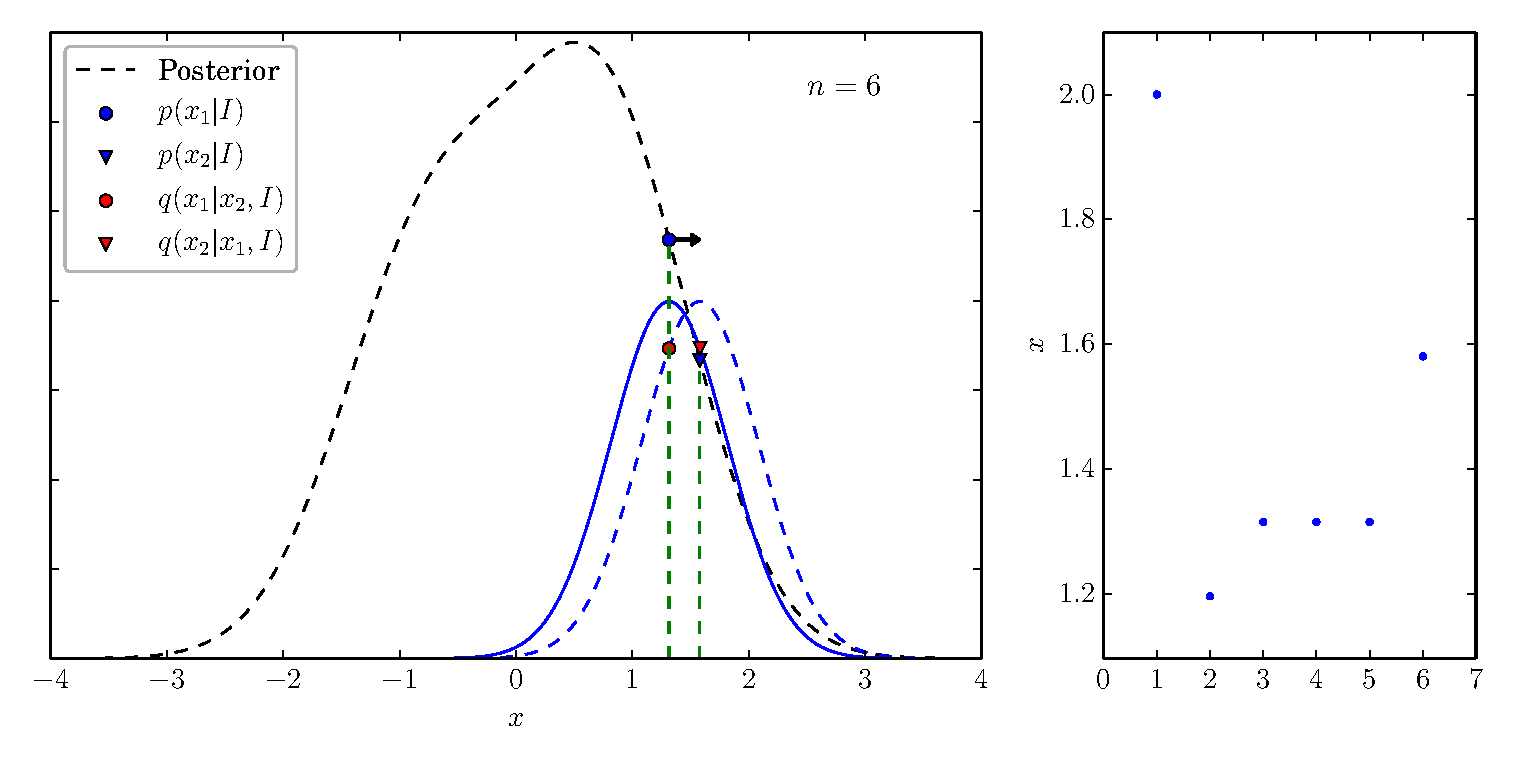
\includegraphics[keepaspectratio,width=\textwidth,height=250pt]{figures/mcmc_example_2.pdf}
\label{mcmc_example_2}
\end{figure}

\end{frame}

\begin{frame}

\frametitle{MCMC demonstration}
\label{mcmcdemonstration}

\begin{figure}[htbp]
\centering
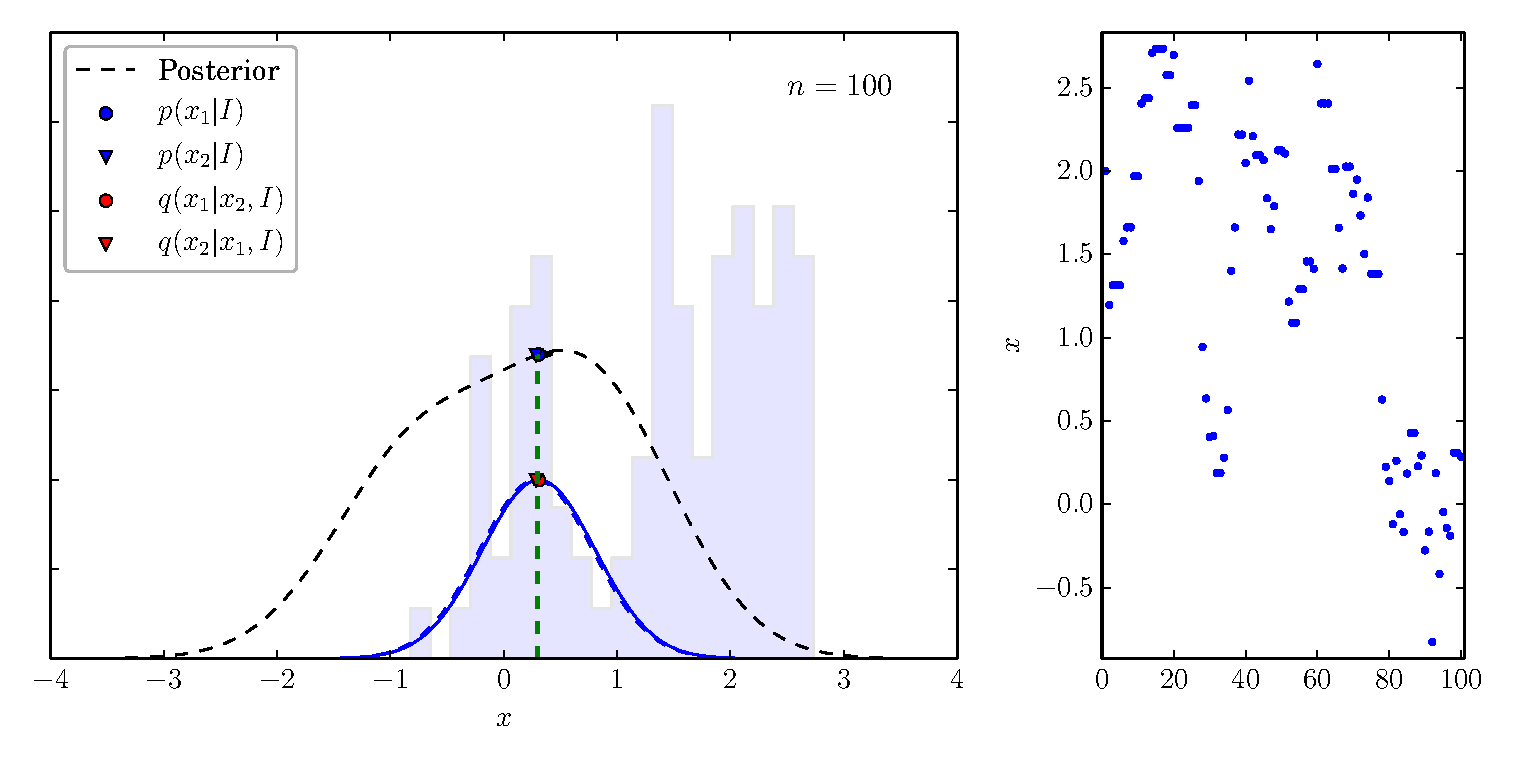
\includegraphics[keepaspectratio,width=\textwidth,height=250pt]{figures/mcmc_example_3.pdf}
\label{mcmc_example_3}
\end{figure}

\end{frame}

\begin{frame}

\frametitle{MCMC demonstration}
\label{mcmcdemonstration}

\begin{figure}[htbp]
\centering
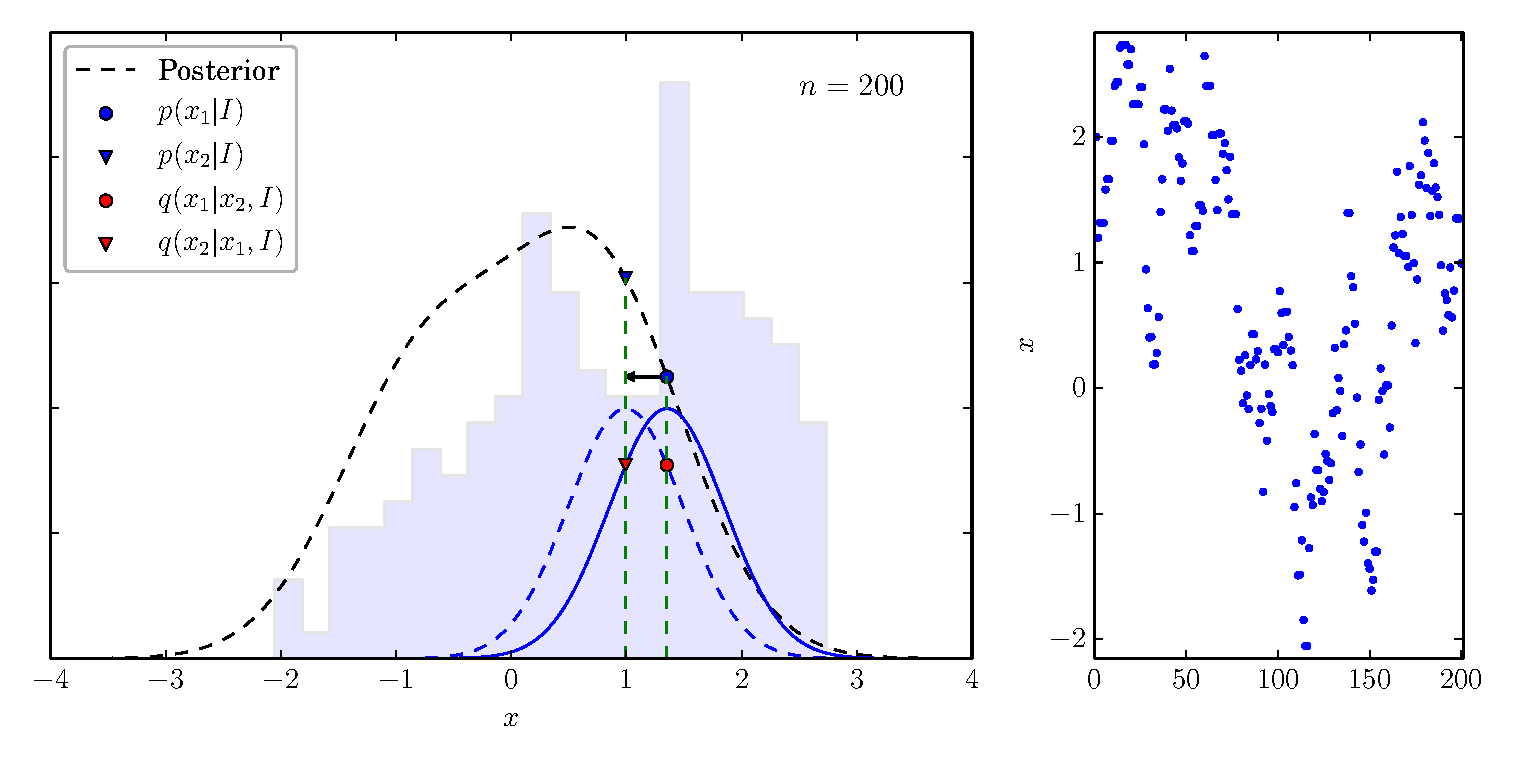
\includegraphics[keepaspectratio,width=\textwidth,height=250pt]{figures/mcmc_example_4.pdf}
\label{mcmc_example_4}
\end{figure}

\end{frame}

\begin{frame}

\frametitle{MCMC demonstration}
\label{mcmcdemonstration}

\begin{figure}[htbp]
\centering
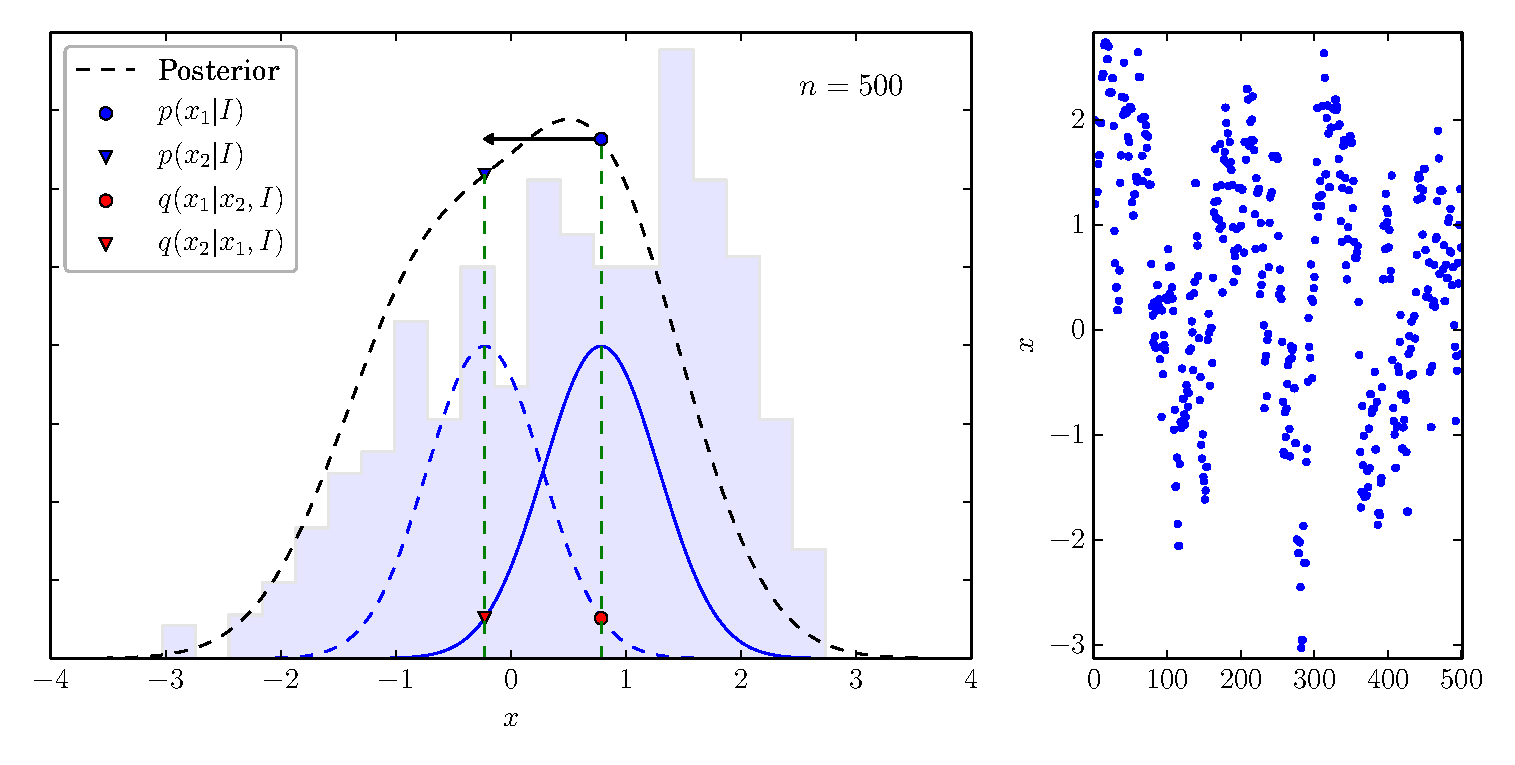
\includegraphics[keepaspectratio,width=\textwidth,height=250pt]{figures/mcmc_example_5.pdf}
\label{mcmc_example_5}
\end{figure}

\end{frame}

\begin{frame}

\frametitle{MCMC demonstration}
\label{mcmcdemonstration}

\begin{figure}[htbp]
\centering
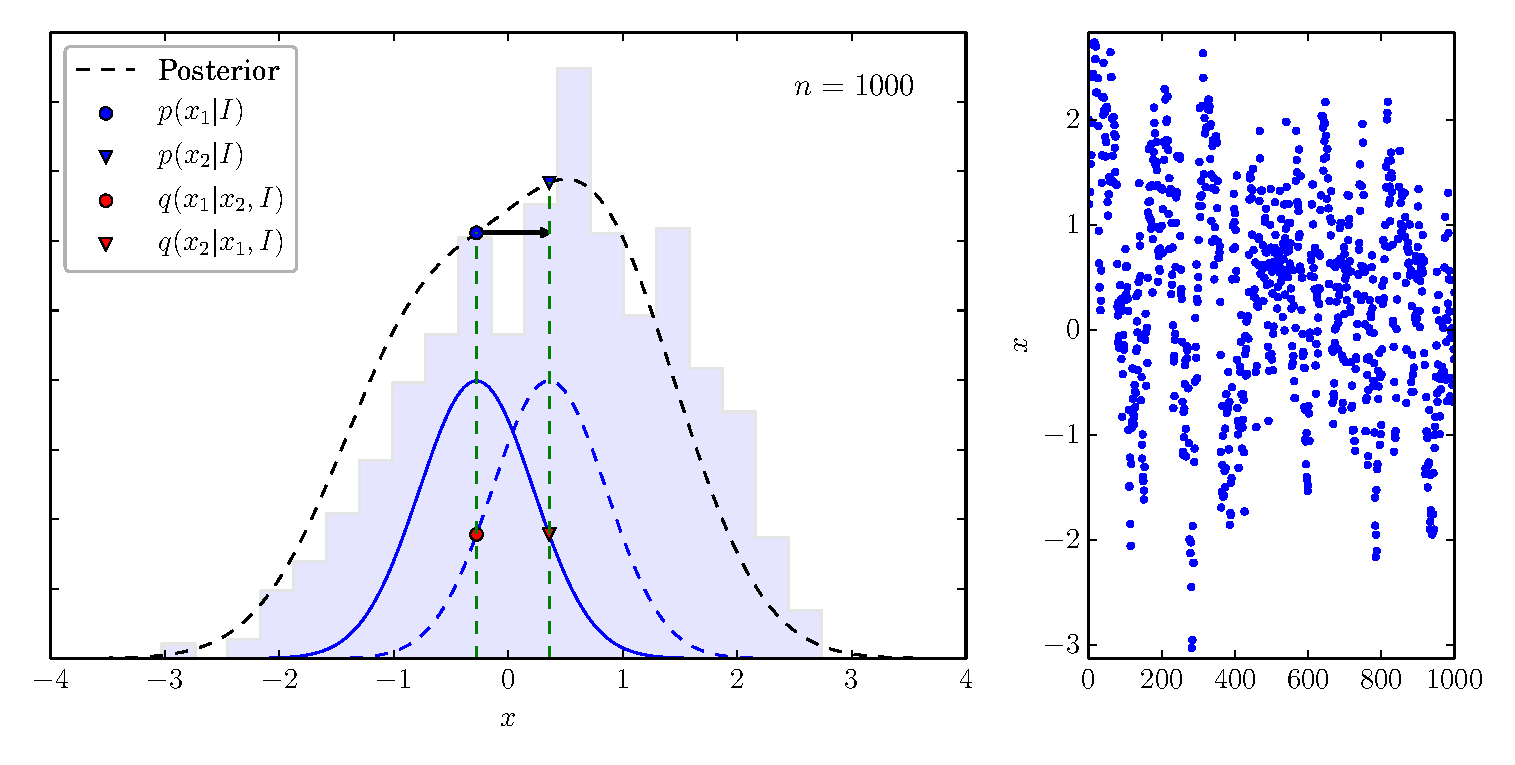
\includegraphics[keepaspectratio,width=\textwidth,height=250pt]{figures/mcmc_example_6.pdf}
\label{mcmc_example_6}
\end{figure}

\end{frame}

\begin{frame}

\frametitle{MCMC demonstration}
\label{mcmcdemonstration}

\begin{figure}[htbp]
\centering
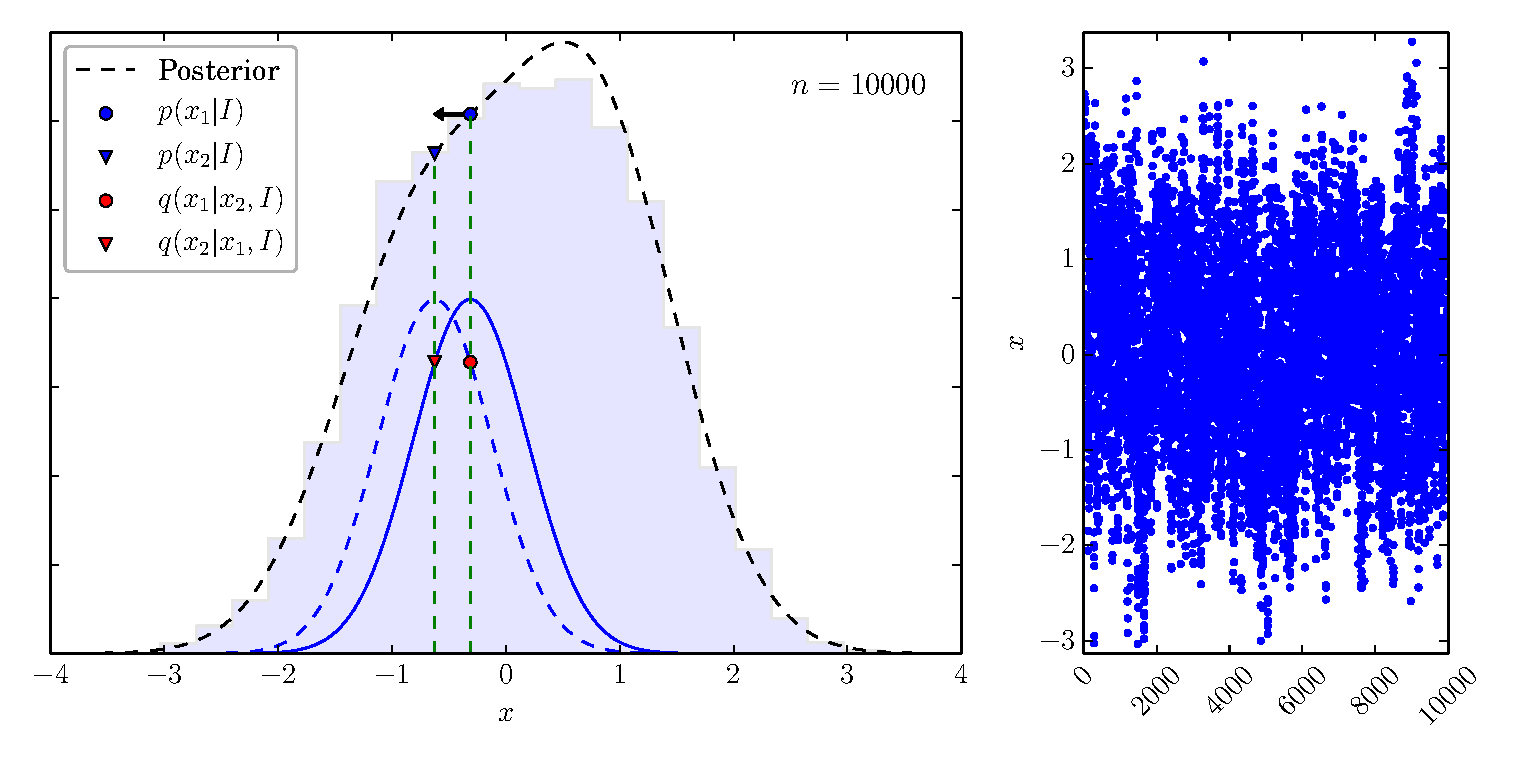
\includegraphics[keepaspectratio,width=\textwidth,height=250pt]{figures/mcmc_example_7.pdf}
\label{mcmc_example_7}
\end{figure}

\end{frame}

\begin{frame}

\frametitle{MCMC demonstration}
\label{mcmcdemonstration}

\begin{figure}[htbp]
\centering
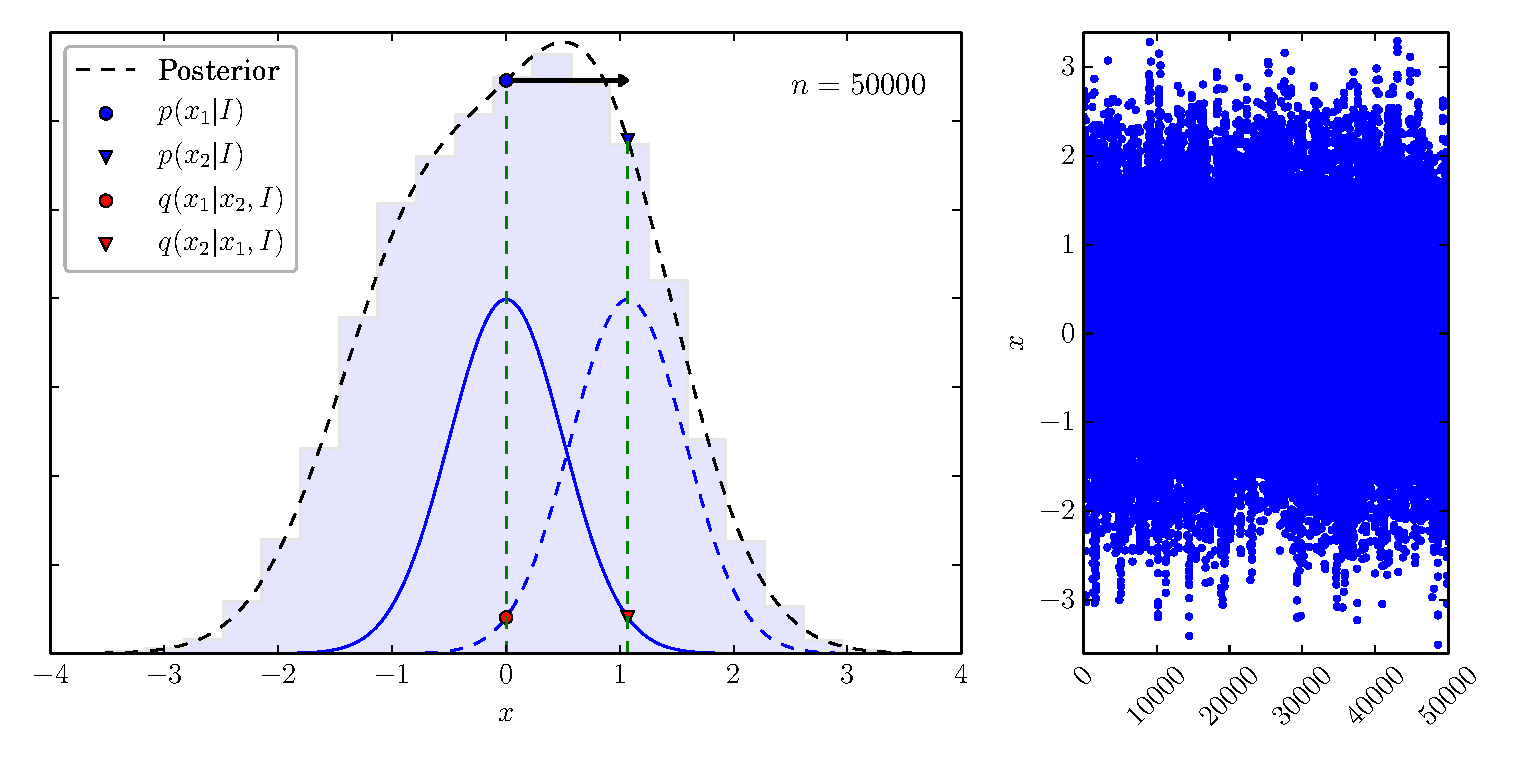
\includegraphics[keepaspectratio,width=\textwidth,height=250pt]{figures/mcmc_example_8.pdf}
\label{mcmc_example_8}
\end{figure}

\end{frame}

\begin{frame}

\frametitle{MCMC tuning}
\label{mcmctuning}

If we don't choose a start point close to the bulk of the posterior it may take time
for the chain to converge on that area, so (given a non-infinite amount of samples)
a number of initial points may need to be \emph{discarded} during the \textbf{burn-in}.

(A couple of) diagnostic \href{http://support.sas.com/documentation/cdl/en/statug/63347/HTML/default/viewer.htm\#statug\_introbayes\_sect008.htm}{methods} to assess convergence are:

\begin{itemize}
\item Geweke's test - test whether the means of an early part of the chain are consistent with the means for a later part

\item Gelman-Rubin test - test whether the variances of two parallel chains are consistent

\end{itemize}

Although just checking by eyeball is often a good way to proceed.

\end{frame}

\begin{frame}

\frametitle{MCMC tuning}
\label{mcmctuning}

MCMC chains are not necessarily uncorrelated (not entirely Markovian!), so you can
calculate the autocorrelation length of the chains and thin them accordingly. This
can also be used as a test of convergence, in that the autocorrelation length may be large
during the burn in phase.

\end{frame}

\begin{frame}

\frametitle{MCMC tuning}
\label{mcmctuning}

If you have an infinite chain (almost) any choice of start position and proposal would
produce the marginalised posterior, but we can only practically produce a finite number
of samples, e.g. $100\,000\text{s}$ or $1\,000\,000\text{s}$

For efficient sampling we could have:

\begin{itemize}
\item a proposal that quite closely matches the posterior being sampled (e.g. via adjusting the proposal during \textbf{burn-in} based on covariance of currently collected samples)

\item use a parameterisation where the parameters are (close to) independent

\item simulated annealing (flattening the likelihood by ``raising the temperature'' during a \textbf{burn-in} period)

\end{itemize}

\end{frame}

\begin{frame}

\frametitle{MCMC tuning}
\label{mcmctuning}

Simple MCMC methods can have problems when:

\begin{itemize}
\item posterior is very tightly constrained within a very small part of the allowed parameter space

\item posterior is multi-modal

\item posterior has oddly shaped degeneracies between parameters

\end{itemize}

(A couple of) methods to address these are e.g.

\begin{itemize}
\item parallel tempering

\item ensemble samplers

\end{itemize}

\end{frame}

\begin{frame}

\frametitle{Further advanced methods}
\label{furtheradvancedmethods}

There are lots of other advanced methods suitable for dealing with more complex situations, e.g.:

\begin{itemize}
\item \href{http://en.wikipedia.org/wiki/Nested_sampling_algorithm}{Nested sampling} (evaluate \emph{evidence} integrals)

\item \href{http://en.wikipedia.org/wiki/Principal_component_analysis}{Principle component analysis (PCA) (data compression)}

\item \href{http://en.wikipedia.org/wiki/Reversible-jump_Markov_chain_Monte_Carlo}{Reversible Jump MCMC}

\item \href{http://en.wikipedia.org/wiki/Bayesian_hierarchical_modeling}{Hierarchical models}

\item \href{http://en.wikipedia.org/wiki/Approximate_Bayesian_computation}{Approximate Bayesian Computation} (ABC)

\item Non-parameteric methods

\begin{itemize}
\item \href{http://en.wikipedia.org/wiki/Kriging}{Gaussian processes}

\item \href{http://en.wikipedia.org/wiki/Dirichlet_process}{Dirichlet processes}

\end{itemize}

\item \href{http://en.wikipedia.org/wiki/Bayesian_network}{Bayesian neural networks}

\end{itemize}

It is a large and rapidly evolving field!

\end{frame}

\mode<all>
\input{mmd-beamer-footer}

\end{document}\mode*

